\documentclass{beamer}
%\documentclass[handout]{beamer}
\usepackage{amsmath}
\usepackage{amssymb}
\usepackage{tikz}
\usetikzlibrary{bayesnet}

\mode<presentation>

\title[]{Correctness of Local Probability Propagation\\in Graphical Models with Loops}
\subtitle{by\\Yair Weiss}
\author{Ben Eyal}

\usetheme{Darmstadt}
\usefonttheme{professionalfonts}

\AtBeginSubsection[]
{
    \begin{frame}<beamer>{Outline}
        \tableofcontents[currentsection,currentsubsection]
    \end{frame}
}

\begin{document}

\begin{frame}
    \titlepage
\end{frame}

\begin{frame}{Outline}
    \tableofcontents
\end{frame}

%%%%%%%%%%%% 1 INTRODUCTION %%%%%%%%%%%%

\section{Introduction}

%%%%%%%%%%%% 1.1 DEFINITIONS %%%%%%%%%%%%

\subsection{Definitions}
\begin{frame}{Breaking Down the Title - Part I}
    \begin{center}
        \Large{Correctness of Local Probability Propagation in \alert<2>{Graphical Models} with Loops}
    \end{center}
\end{frame}
\begin{frame}{Probabilistic Graphical Models}
    \pause
    \begin{definition}
        A Probabilistic Graphical Model (PGM) is a graph, either directed or undirected, in which the nodes correspond to random variables,
        and the edges correspond to direct probabilistic interactions between them.
    \end{definition}
\end{frame}
\begin{frame}{Probabilistic Graphical Models}
    \pause
    \begin{definition}
        A \textbf{Bayes network} is a directed acyclic PGM whose edges can be seen as ``cause'' and ``effect'', e.g. an
        edge $ X \rightarrow Y $ means that $ X $ directly influences $ Y $, or ``$ X $ is the cause of $ Y $''.
    \end{definition}
    \pause
    \begin{center}
        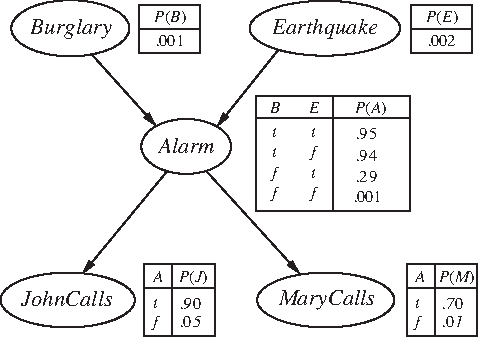
\includegraphics[scale=0.75]{burglary2}\\
    \end{center}
\end{frame}
\begin{frame}{Probabilistic Graphical Models}
    \pause
    \begin{definition}
        A Markov Random Field (MRF), or a \textbf{Markov network}, is an undirected PGM which is used when the relations between
        random variables are symmetric, rather than hierarchical, e.g. pixels in an image.
    \end{definition}
    \pause
    \begin{columns}
        \begin{column}[t]{0.2 \textwidth}
            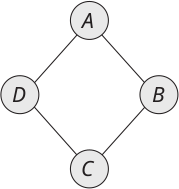
\includegraphics[scale=0.4]{mrf1}
        \end{column}
        \begin{column}[t]{0.8 \textwidth}
            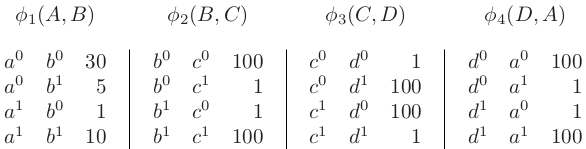
\includegraphics[scale=0.4]{mrf2}
        \end{column}
    \end{columns}
\end{frame}
\begin{frame}{Breaking Down the Title - Part II}
    \begin{center}
        \Large{Correctness of \alert<2>{Local Probability Propagation} in \alert<1>{Graphical Models} with Loops}
    \end{center}
\end{frame}
\begin{frame}{Reminder}
    \begin{block}{Conditional Probability}
        \[ \Pr \left( A \mid B \right) = \frac{\Pr \left( A, B \right)}{\Pr \left( B \right)} \]
    \end{block}
    \pause
    \begin{block}{Bayes' Theorem}
        Bayes' theorem gives us the relation between the \alert{posterior~probability}, $ \Pr \left( A \mid B \right) $, and the \alert{prior probability}, $ \Pr \left( A \right) $.
        \[ \Pr \left( A \mid B \right) = \frac{\Pr \left( B \mid A \right) \Pr \left( A \right)}{\Pr \left( B \right)} \]
    \end{block}
\end{frame}
\begin{frame}{Reminder}
    \pause
    \begin{block}{Marginal Probability}
        Given a joint probability distribution $ \Pr \left( X, Y \right) $,
        \begin{align*}
            \Pr \left( X = x \right) &= \sum_{y} \Pr \left( X = x, Y = y \right) \\
                                     &= \sum_{y} \Pr \left( X = x \mid Y = y \right) \Pr \left( Y = y \right)
        \end{align*}
        is the \alert{marginal distribution} of $ X $.
    \end{block}
\end{frame}
\begin{frame}{Belief Propagation}
    \begin{block}{The Task of Inference}
        Inference is divided into three subtasks:
        \pause
        \begin{itemize}[<+->]
            \item \emph{Marginalization}: Calculating the marginal probability of a variable given the observed variables -- e.g. $ \Pr \left( C = c \mid \mathcal{O} \right) $.
            \item \emph{Maximum a posteriori (MAP) assignment}: Finding assignments to the unobserved variables that are most probable given the observed variables -- e.g. finding $ \left( b, c, d, e \right) $ such that $ \Pr \left( B = b, C = c, D = d, E = e \mid \mathcal{O} \right) $ is maximized.
            \item \emph{Maximum Marginal (MM) assignment}: Finding assignments to the unobserved variables that maximize the marginal probability of the assignment -- e.g. finding $ \left( b, c, d, e \right) $ such that $ \Pr \left( B = b \mid \mathcal{O} \right) $,
            $ \Pr \left( C = c \mid \mathcal{O} \right) $, $ \Pr \left( D = d \mid \mathcal{O} \right) $, $ \Pr \left( E = e \mid \mathcal{O} \right) $ are all maximized.
        \end{itemize}
    \end{block}
\end{frame}
\begin{frame}{Belief Propagation}
    \begin{definition}
        Belief Propagation (Pearl, 1982) is an iterative message-passing algorithm used to perform inference on PGMs.\\
        The algorithm gives exact marginals on polytrees (a directed graph with only a single path between any two nodes).
    \end{definition}
\end{frame}
\begin{frame}{Example}
    \pause
    \begin{center}
        
\includegraphics[scale=0.1]{warning}
    \end{center}
\end{frame}
\begin{frame}{Example}
    \pause
    We would like to compute the maximum marginal probability $ \Pr \left( X = x_{1} \mid Y \right) $ given the following Markov network:
    \begin{figure}[h]
        \centering
        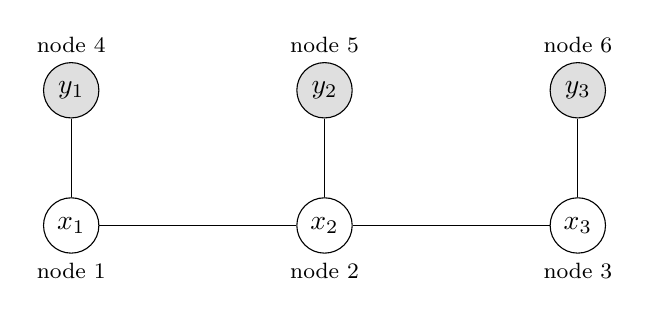
\begin{tikzpicture}
        
        % Nodes
        
        \node[obs, label=above:node 4] (y1) {$ y_{1} $};
        \node[obs, right=2.5 of y1, label=above:node 5] (y2) {$ y_{2} $};
        \node[obs, right=2.5 of y2, label=above:node 6] (y3) {$ y_{3} $};
        \node[latent, below=of y1, label=below:node 1] (x1) {$ x_{1} $};
        \node[latent, right=of x1, below=of y2, label=below:node 2] (x2) {$ x_{2} $};
        \node[latent, right=of x2, below=of y3, label=below:node 3] (x3) {$ x_{3} $};
        
        % Edges
        
        \edge[-] {y1} {x1};
        \edge[-] {y2} {x2};
        \edge[-] {y3} {x3};
        \edge[-] {x1} {x2};
        \edge[-] {x2} {x3};
        
        \end{tikzpicture}
    \end{figure}
\end{frame}
\begin{frame}{Example}
    \pause
    If we knew nothing about the structure of the joint probability:
    \[ \Pr \left( X = x_{1} \mid Y \right) = \sum_{x_{2}} \sum_{x_{3}} \Pr \left( x_{1}, x_{2}, x_{3} \mid Y \right) \]
    \pause
    This might not look like much, but the time complexity increases exponentially with the number of unobserved variables.\\
    \pause
    Did I mention that both exact and approximate inference are hard? \pause As in $ \mathcal{NP} $-hard?
\end{frame}
\begin{frame}{Example}
    Lucky for us, we do know something about the structure of the joint probability! \pause
    \[
        {\scriptstyle \Pr \left( x_{1} \mid Y \right) = \frac{1}{\Pr \left( Y \right)}
        \sum_{x_{2}} \sum_{x_{3}}
        \phi_{12}\left( x_{1}, x_{2} \right) \phi_{23}\left( x_{2}, x_{3} \right)
        \psi_{1}\left( y_{1}, x_{1} \right) \psi_{2}\left( y_{2}, x_{2} \right) \psi_{3}\left( y_{3}, x_{3} \right)}
    \]
    \pause
    Do not despair! This is going to be very clear -- very quick.
\end{frame}
\begin{frame}{Example}
    \begin{onlyenv}<1>
        \[
            {\scriptstyle \Pr \left( x_{1} \mid Y \right) = \frac{1}{\Pr \left( Y \right)}
            \sum_{x_{2}} \sum_{x_{3}}
            \phi_{12}\left( x_{1}, x_{2} \right) \phi_{23}\left( x_{2}, x_{3} \right)
            \psi_{1}\left( y_{1}, x_{1} \right) \psi_{2}\left( y_{2}, x_{2} \right) \psi_{3}\left( y_{3}, x_{3} \right)}
        \]
        \begin{figure}[h]
            \centering
            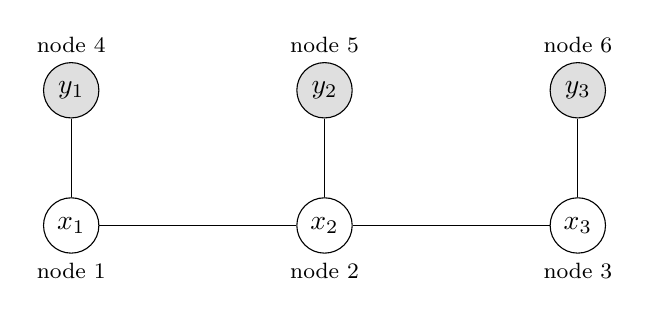
\begin{tikzpicture}
            
            % Nodes
            
            \node[obs, label=above:node 4] (y1) {$ y_{1} $};
            \node[obs, right=2.5 of y1, label=above:node 5] (y2) {$ y_{2} $};
            \node[obs, right=2.5 of y2, label=above:node 6] (y3) {$ y_{3} $};
            \node[latent, below=of y1, label=below:node 1] (x1) {$ x_{1} $};
            \node[latent, right=of x1, below=of y2, label=below:node 2] (x2) {$ x_{2} $};
            \node[latent, right=of x2, below=of y3, label=below:node 3] (x3) {$ x_{3} $};
            
            % Edges
            
            \edge[-] {y1} {x1};
            \edge[-] {y2} {x2};
            \edge[-] {y3} {x3};
            \edge[-] {x1} {x2};
            \edge[-] {x2} {x3};
            
            \end{tikzpicture}
        \end{figure}
    \end{onlyenv}
    \begin{onlyenv}<2>
        \[
            {\scriptstyle \Pr \left( x_{1} \mid Y \right) = \frac{1}{\Pr \left( Y \right)}
            \psi_{1}\left( y_{1}, x_{1} \right)
            \sum_{x_{2}} \phi_{12}\left( x_{1}, x_{2} \right) \psi_{2}\left( y_{2}, x_{2} \right)
            \sum_{x_{3}} \phi_{23}\left( x_{2}, x_{3} \right) \psi_{3}\left( y_{3}, x_{3} \right)}
        \]
        \begin{figure}[h]
            \centering
            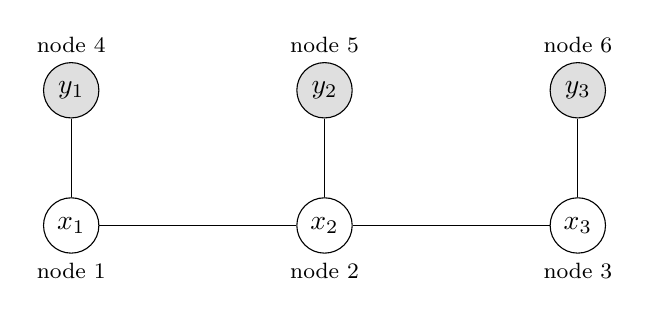
\begin{tikzpicture}
            
            % Nodes
            
            \node[obs, label=above:node 4] (y1) {$ y_{1} $};
            \node[obs, right=2.5 of y1, label=above:node 5] (y2) {$ y_{2} $};
            \node[obs, right=2.5 of y2, label=above:node 6] (y3) {$ y_{3} $};
            \node[latent, below=of y1, label=below:node 1] (x1) {$ x_{1} $};
            \node[latent, right=of x1, below=of y2, label=below:node 2] (x2) {$ x_{2} $};
            \node[latent, right=of x2, below=of y3, label=below:node 3] (x3) {$ x_{3} $};
            
            % Edges
            
            \edge[-] {y1} {x1};
            \edge[-] {y2} {x2};
            \edge[-] {y3} {x3};
            \edge[-] {x1} {x2};
            \edge[-] {x2} {x3};
            
            \end{tikzpicture}
        \end{figure}
    \end{onlyenv}
    \begin{onlyenv}<3>
        \[
            {\scriptstyle \Pr \left( x_{1} \mid Y \right) = \frac{1}{\Pr \left( Y \right)}
            m_{41}\left( x_{1} \right)
            \sum_{x_{2}} \phi_{12}\left( x_{1}, x_{2} \right) m_{52}\left( x_{2} \right)
            \sum_{x_{3}} \phi_{23}\left( x_{2}, x_{3} \right) m_{63}\left( x_{3} \right)}
        \]
        \begin{figure}[h]
            \centering
            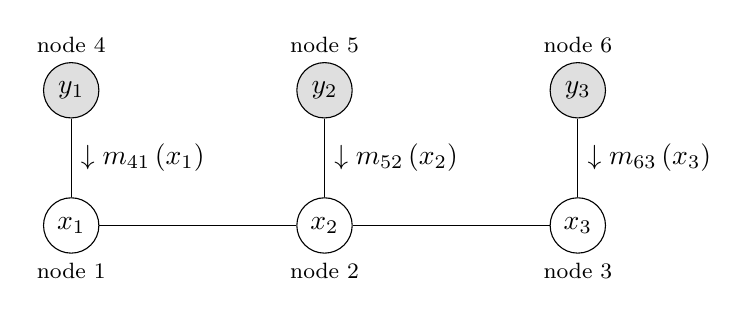
\begin{tikzpicture}
            
            % Nodes
            
            \node[obs, label=above:node 4] (y1) {$ y_{1} $};
            \node[obs, right=2.5 of y1, label=above:node 5] (y2) {$ y_{2} $};
            \node[obs, right=2.5 of y2, label=above:node 6] (y3) {$ y_{3} $};
            \node[latent, below=of y1, label=below:node 1] (x1) {$ x_{1} $};
            \node[latent, right=of x1, below=of y2, label=below:node 2] (x2) {$ x_{2} $};
            \node[latent, right=of x2, below=of y3, label=below:node 3] (x3) {$ x_{3} $};
            
            % Message Labels
            
            \draw (y1) -- (x1) node [midway, right, fill=white] {$ \downarrow m_{41} \left( x_{1} \right) $};
            \draw (y2) -- (x2) node [midway, right, fill=white] {$ \downarrow m_{52} \left( x_{2} \right) $};
            \draw (y3) -- (x3) node [midway, right, fill=white] {$ \downarrow m_{63} \left( x_{3} \right) $};
            
            % Edges
            
            \edge[-] {y1} {x1};
            \edge[-] {y2} {x2};
            \edge[-] {y3} {x3};
            \edge[-] {x1} {x2};
            \edge[-] {x2} {x3};
            
            \end{tikzpicture}
        \end{figure}
    \end{onlyenv}
    \begin{onlyenv}<4>
        \[
            {\scriptstyle \Pr \left( x_{1} \mid Y \right) = \frac{1}{\Pr \left( Y \right)}
            m_{41}\left( x_{1} \right)
            \sum_{x_{2}} \phi_{12}\left( x_{1}, x_{2} \right) m_{52}\left( x_{2} \right) m_{32}\left( x_{2} \right) }
        \]
        \begin{figure}[h]
            \centering
            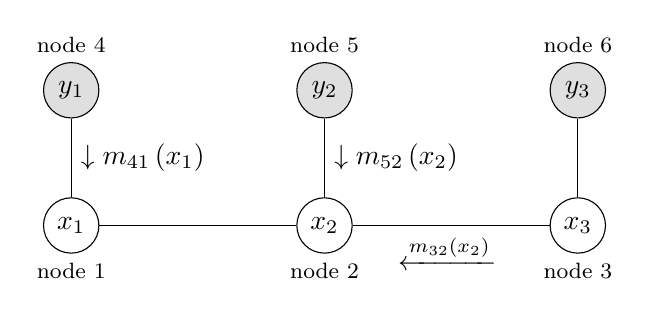
\begin{tikzpicture}
            
            % Nodes
            
            \node[obs, label=above:node 4] (y1) {$ y_{1} $};
            \node[obs, right=2.5 of y1, label=above:node 5] (y2) {$ y_{2} $};
            \node[obs, right=2.5 of y2, label=above:node 6] (y3) {$ y_{3} $};
            \node[latent, below=of y1, label=below:node 1] (x1) {$ x_{1} $};
            \node[latent, right=of x1, below=of y2, label=below:node 2] (x2) {$ x_{2} $};
            \node[latent, right=of x2, below=of y3, label=below:node 3] (x3) {$ x_{3} $};
            
            % Message Labels

            \draw (y1) -- (x1) node [midway, right, fill=white] {$ \downarrow m_{41} \left( x_{1} \right) $};
            \draw (y2) -- (x2) node [midway, right, fill=white] {$ \downarrow m_{52} \left( x_{2} \right) $};
            \draw (x3) -- (x2) node [midway, below, fill=white] {$ \xleftarrow {m_{32} \left( x_{2} \right)} {} $};
            
            % Edges
            
            \edge[-] {y1} {x1};
            \edge[-] {y2} {x2};
            \edge[-] {y3} {x3};
            \edge[-] {x1} {x2};
            \edge[-] {x2} {x3};
            
            \end{tikzpicture}
        \end{figure}
    \end{onlyenv}
    \begin{onlyenv}<5>
        \[
            {\scriptstyle \Pr \left( x_{1} \mid Y \right) = \frac{1}{\Pr \left( Y \right)}
            m_{41}\left( x_{1} \right) m_{21}\left( x_{1} \right) }
        \]
        \begin{figure}[h]
            \centering
            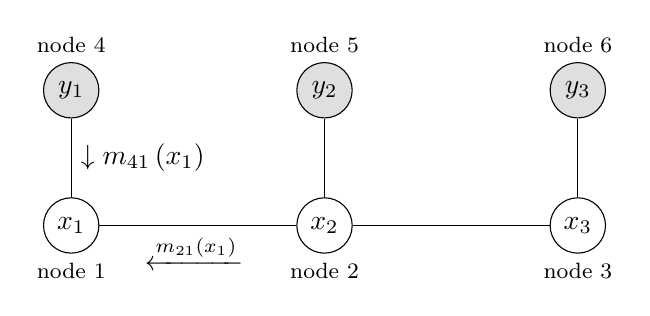
\begin{tikzpicture}
            
            % Nodes
            
            \node[obs, label=above:node 4] (y1) {$ y_{1} $};
            \node[obs, right=2.5 of y1, label=above:node 5] (y2) {$ y_{2} $};
            \node[obs, right=2.5 of y2, label=above:node 6] (y3) {$ y_{3} $};
            \node[latent, below=of y1, label=below:node 1] (x1) {$ x_{1} $};
            \node[latent, right=of x1, below=of y2, label=below:node 2] (x2) {$ x_{2} $};
            \node[latent, right=of x2, below=of y3, label=below:node 3] (x3) {$ x_{3} $};

            % Message Labels

            \draw (y1) -- (x1) node [midway, right, fill=white] {$ \downarrow m_{41} \left( x_{1} \right) $};
            \draw (x2) -- (x1) node [midway, below, fill=white] {$ \xleftarrow {m_{21} \left( x_{1} \right)} {} $};

            % Edges
            
            \edge[-] {y1} {x1};
            \edge[-] {y2} {x2};
            \edge[-] {y3} {x3};
            \edge[-] {x1} {x2};
            \edge[-] {x2} {x3};
            
            \end{tikzpicture}
        \end{figure}
    \end{onlyenv}
\end{frame}
\begin{frame}{Belief Propagation}
    \pause
    \begin{block}{Inside Belief Propagation}
        In Belief Propagation, every iteration is called \alert{belief update (BU)}. In belief update, the message
        that node $ X $ sends to node $ Y $ is updated as follows:
        \pause
        \begin{enumerate}[<+->]
            \item Combine all messages coming into $ X $ except for that coming from $ Y $ into a vector $ \vec{v} $. The combination is done by multiplying all the message vectors element by element.
            \item Multiply $ \vec{v} $ by the matrix $ M_{XY} $ corresponding to the link from $ X $ to $ Y $.
            \item Normalize the product $ M_{XY}\vec{v} $ so it sums to $ 1 $. The normalized vector is sent to $ Y $.
        \end{enumerate}
        \visible<5>{The belief vector for a node $ X $ is obtained by combining all incoming messages to $ X $ and normalizing.}
    \end{block}
\end{frame}
\begin{frame}{Belief Propagation}
    \begin{block}{Maximum A-Posteriori (MAP) Assignment Using Belief Propagation}
        To find a MAP assignment, we use the algorithm above, with a small change:\\
        Instead of using matrix multiplication (a sum-of-products), we take the $ \operatorname{argmax} $, giving us a max-of-products.\\
        This step is called \alert{belief revision (BR)}.
    \end{block}
\end{frame}

%%%%%%%%%%%% 1.2 THE PROBLEM %%%%%%%%%%%%

\subsection{The Problem}
\begin{frame}{Breaking Down the Title - Part III}
    \begin{center}
        \Large{Correctness of \alert<1>{Local Probability Propagation} in Graphical Models with \alert<2>{Loops}}
    \end{center}
\end{frame}
\begin{frame}{``Loopy'' Belief Propagation}
    \begin{block}{Belief Propagation on General Graphs}
        As we have already seen, Belief Propagation is guaranteed to converge on the exact marginals or MAP assignments given a singly-connected graph.\\
        What happens when we have loops?
        \pause
        \begin{itemize}[<+->]
            \item Divergence
            \item Fluctuations between different values
            \item Convergence on the wrong values
        \end{itemize}
        \visible<5-6>{Theoretically...\\}
        \visible<6>{In practice, ``loopy'' Belief Propagation is doing surprisingly well!}
    \end{block}
\end{frame}
\section{Belief Propagation on PGMs with a Single Loop}
\subsection{Correctness}
\begin{frame}{Breaking Down the Title - Finale}
    \begin{center}
        \Large{\alert<2>{Correctness} of Local Probability Propagation in Graphical Models with \alert<1>{Loops}}
    \end{center}
\end{frame}
\begin{frame}
    \begin{block}{Theory vs. Practice}
        Although Loopy Belief Propagation is doing great in some cases, the theoretical problems shown earlier do arise.\\
        \pause We wish to know when Loopy Belief Propagation is guaranteed to converge.\\
        \pause In his paper, Weiss proves that given a PGM with a single loop:
        \pause
        \begin{itemize}[<+->]
            \item belief revision in Loopy Belief Propagation will always converge on a correct MAP assignment.
            \item belief update will converge on a marginal that is not the correct marginal, but is closely related to it.
        \end{itemize}
    \end{block}
\end{frame}
\begin{frame}
    \begin{block}{Motivation}
        The problem with loops is what Weiss refers to as ``double counting'':
        \pause
        \begin{center}
            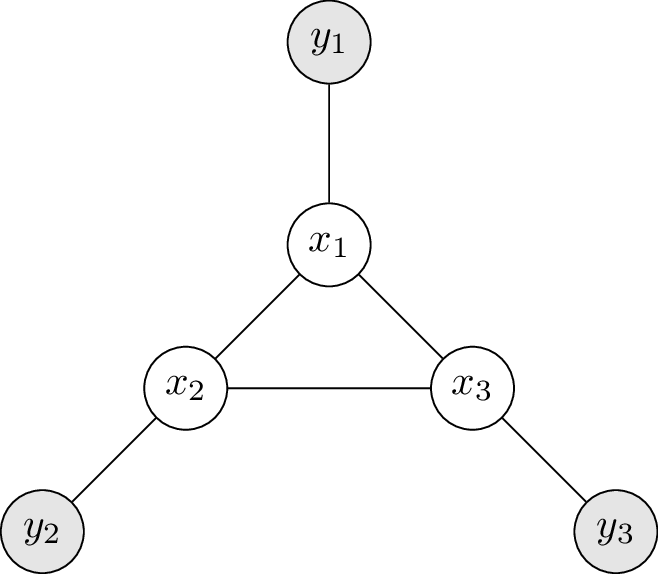
\includegraphics[scale=0.7]{fig}
        \end{center}
        \pause
        In a graph with a single loop, Weiss shows this ``double counting'' is guaranteed to occur equally among all nodes in the loop, therefore still reaching convergence.
    \end{block}    
\end{frame}
\section{Conclusion}
\subsection{What Have We Achieved?}
\begin{frame}
    \pause
    \begin{itemize}[<+->]
        \item We can define a Probabilistic Graphical Model (PGM), and name two specific types.
        \item We know what are prior and posterior probabilities, and how Bayes' theorem connects them.
        \item We can trace the steps of the Belief Propagation algorithm.
        \item We are not afraid of phrases such as ``sum-product'', ``max-product'', or ``message-passing''.
        \item We are aware of three problems that may arise in PGMs with loops...
        \item ...but we also know that loops are not always a problem in practice.
        \item We know what to expect when running Loopy Belief Propagation on a PGM with a single loop.
    \end{itemize}
\end{frame}
\subsection{The End}
\begin{frame}
    \begin{center}
        \Huge{Thank you for your time!}\\~\\
        \pause
        \LARGE{Questions?}
    \end{center}
\end{frame}
\end{document}